\documentclass{ieeetj}
\newcommand{\seclogo}{}
\usepackage{cite}
\usepackage{amsmath,amssymb,amsfonts}
\usepackage{listings}
\usepackage{algorithmic}
\usepackage{graphicx,color}
\usepackage{textcomp}
\usepackage{hyperref}
\usepackage{float}
\usepackage[table,xcdraw]{xcolor}
\definecolor{blau}{RGB}{198, 220, 255} 
\definecolor{gris}{RGB}{176, 176, 176}
\definecolor{verd}{RGB}{ 173, 240, 199}

\hypersetup{hidelinks=true}
\usepackage{algorithm,algorithmic}
\lstset{
    language=Java,
    basicstyle=\ttfamily\small,
    keywordstyle=\bfseries\color{blue},
    stringstyle=\color{red},
    morecomment=[l][\color{magenta}]{//},
    frame=single,
    breaklines=true,
    showstringspaces=false,
    tabsize=1,
}
\def\BibTeX{{\rm B\kern-.05em{\sc i\kern-.025em b}\kern-.08em
    T\kern-.1667em\lower.7ex\hbox{E}\kern-.125emX}}
\AtBeginDocument{\definecolor{tmlcncolor}{cmyk}{0.93,0.59,0.15,0.02}\definecolor{NavyBlue}{RGB}{0,86,125}}

% Definim el logo
\def\OJlogo{
    \vspace{-14pt} % Espai negatiu per pujar el logo
    
\includegraphics[height=0.96cm]{png/logo.png}}

\begin{document}
\receiveddate{29 Abril, 2025}
\publisheddate{27 Maig, 2025}
\currentdate{27 Maig, 2025}

\title{Programació dinàmica: COMPARADOR D'IDIOMES}

\author{Josep Ferriol, Daniel García, Khaoula Ikkene, Biel Perelló} \affil{Universitat de les Illes Balears, Departament d'Enginyeria Informàtica} \corresp{Autor de contacte: Daniel García (email: daniel.garcia19@estudiant.uib.es)}



\begin{abstract} 
Aquest document presenta el desenvolupament d'una aplicació en llenguatge Java per al càlcul de distàncies entre un conjunt d'idiomes indoeuropeus\cite{IndoEuropeanLanguages}.

L'objectiu principal del programa és implementar l'algorisme dinàmic de Levenshtein\cite{LevenshteinDistance} i adaptar-lo per al càlcul de distàncies lingüístiques entre diverses llengües. Les dues preguntes fonamentals que el nostre programa ha de ser capaç de respondre són:\newline
Seleccionant un idioma, a quina distància es troba un altre idioma?\newline
Seleccionant un idioma, a quina distància es troben tots els altres?\newline

Com a funcionalitats opcionals, s'ha implementat la possibilitat de comparar tots els idiomes entre si per obtenir una visió global de les distàncies. A nivell visual, s'han implementat les tres gràfiques recomanades a l'enunciat: Diagrama de barres, Arbre de distàncies, i l'Arbre filo-lèxic.

Els recursos emprats per calcular les distàncies són els diccionaris propis de cada llengua. No obstant això, donat que el càlcul pot ser massa lent quan es requereix una resposta immediata, s'han implementat dues funcionalitats addicionals per optimitzar el procés: \newline
La possibilitat d'importar i exportar les dades de les distàncies ja calculades per reutilitzar-les sense necessitat de recalcular-les.\newline
L'ús del \textbf{probabilisticWrapper}, una tècnica que permet obtenir estimacions de distàncies de manera més eficient en determinades situacions.\newline

Aquestes dues funcionalitats, juntament amb la resta d'implementacions, seran detallades en aquest document.

\end{abstract}

\begin{IEEEkeywords}
Programació dinàmica, distància de Levenshtein, MVC, ExecutorService, Java Swing Arbre filo-lèxic, graf de distàncies, probabilisitcWrapper, Monte Carlo 
\end{IEEEkeywords}


\maketitle


\section{Introducció}
La comparació automàtica d’idiomes és un problema interessant tant en l’àmbit de la lingüística com en el de l’enginyeria informàtica. Disposar d’una mesura quantitativa de la semblança o diferència entre dos idiomes pot ajudar a visualitzar-ne el grau de parentiu o a avaluar la dificultat de traducció entre ells. En aquest projecte s’ha desenvolupat una aplicació anomenada \emph{Comparador d’Idiomes} capaç de calcular una distància numèrica entre idiomes a partir del seu lèxic i de presentar els resultats de forma intuïtiva a l’usuari.\newline

L’objectiu principal del projecte és implementar un algoritme eficient per calcular la \textbf{distància lèxica} entre dues llengües, és a dir, una mesura de com diferent és el vocabulari de dos idiomes. Per a això s’utilitza la \textbf{distància d’edició de Levenshtein}, un algoritme de programació dinàmica conegut per calcular el nombre mínim d’operacions necessàries per transformar una paraula en una altra. La motivació de l’ús d’aquest algoritme és que permet quantificar la diferència entre paraules de manera robusta, i agregant aquesta diferència al llarg de moltes paraules es pot obtenir una estimació de la distància global entre idiomes. Cal destacar que la distància de Levenshtein s’ha emprat en lingüística per quantificar la distància entre llengües i la correlació amb la intel·ligibilitat mútua \cite{levDistanceWiki}.\newline

A més de l’algorisme base, el projecte incorpora \textbf{tècniques de concurrència} per accelerar els càlculs. Comparar cada parell d’idiomes implica processar grans volums de dades (llistes de paraules) i realitzar molts càlculs de distàncies entre cadenes. 
Per evitar que l’aplicació resulti lenta o que la interfície gràfica es bloquegi durant els càlculs, s’han introduït fils d’execució múltiples que treballen en paral·lel \cite{oracleExecutorService}. D’aquesta manera es pot aprofitar els processadors multicore i mantenir la responsivitat de la interfície d’usuari.\newline

El desenvolupament s’ha realitzat en Java, seguint l’arquitectura \textbf{Model-Vista-Controlador (MVC)}. Aquesta arquitectura facilita la modularitat i manteniment del codi, separant la lògica de càlcul (model), la interfície gràfica d’usuari (vista) i la coordinació de les accions (controlador) \cite{MVC_Theory}\cite{mvcPattern}. \newline L’aplicació resultant permet a l’usuari seleccionar un parell d’idiomes o bé calcular totes les distàncies entre un conjunt d’idiomes alhora, mostrant els resultats en forma de matriu de distàncies i diverses visualitzacions gràfiques (un arbre de distàncies, un arbre filo-lèxic i un diagrama de barres comparatives).


\section{Marc teòric} 
En aquest apartat es descriuen els fonaments teòrics necessaris per entendre el projecte, abastant des de conceptes d’algorismes de comparació de cadenes fins a aspectes d’arquitectura de programari i execució concurrent a Java.

\subsection{Programació Dinàmica}
La \emph{programació dinàmica} és una tècnica de disseny d’algorismes que soluciona problemes dividint-los en subproblemes més petits i reutilitzant els resultats parcials per evitar càlculs redundants \cite{DPConcept}.  
Aquest enfocament s’aplica quan un problema exhibeix \emph{optimal substructure} i \emph{subproblem overlap}, permetent una implementació eficient tant en temps com en memòria.

\subsection{Algorisme de Levenshtein}
La \textbf{distància d’edició de Levenshtein} mesura el nombre mínim d’operacions (inserció, eliminació, substitució) necessàries per transformar una cadena en una altra \cite{levDistanceWiki}.  
S’implementa mitjançant una matriu de costums \(dp[0..n][0..m]\), on

\[
\begin{aligned}
dp[i][j] = \min \bigl\{ &\ dp[i-1][j] + 1,\; \\
                        &\ dp[i][j-1] + 1,\; \\
                        &\ dp[i-1][j-1] + \mathbf{1}_{s_1[i]\neq s_2[j]}, \dots
\bigr\}
\end{aligned}
\]

i es retorna \(dp[n][m]\). La complexitat és \(O(nm)\).

\subsection{Distància Lèxica entre Idiomes}
Per quantificar la diferència entre dos llengües \(A\) i \(B\), definim la distància dirigida
\[
d(A\!\to\!B)
=
\frac{1}{|L_A|}
\sum_{w\in L_A}
\min_{x\in L_B}
\frac{\mathrm{Lev}(w,x)}{\max(|w|,|x|)}
\]
i la distància simètrica
\[
D(A,B)
=
\sqrt{\,d(A\!\to\!B)^2 + d(B\!\to\!A)^2\,},
\]
garantint \(D(A,B)=D(B,A)\).

\subsection{Concurrència i Model d’Execució en Java}
Per accelerar el càlcul de milions de comparacions de cadenes, s’utilitza la biblioteca \texttt{java.util.concurrent} de Java:  
\begin{itemize}
  \item \texttt{ExecutorService} i \texttt{ThreadPoolExecutor} per gestionar pools de fils \cite{oracleExecutorService}.  
  \item Divisió de tasques: càlcul paral·lel de \(d(A\!\to\!B)\) i \(d(B\!\to\!A)\), i subdivisió del conjunt de paraules en blocs processats concurrentment.  
  \item Cancel·lació i sincronització mitjançant \texttt{shutdown()} i variables de control, assegurant que la GUI roman responsiva.
\end{itemize}

\section{Entorn de Programació}

Per dur a terme el desenvolupament d’aquesta pràctica, s’ha utilitzat un conjunt d’eines i tecnologies que han proporcionat un entorn robust i eficient. A continuació es detallen les eines principals emprades:

\begin{itemize}
    \item \textbf{Llenguatge de programació: Java} – El projecte s’ha desenvolupat íntegrament en Java. Java és un llenguatge de programació orientat a objectes reconegut per la seva estabilitat, portabilitat i àmplia col·lecció de llibreries estàndard. L’ús de Java ha permès escriure codi mantenible i independent de la plataforma, executant-se sobre la màquina virtual Java (JVM) en diversos sistemes operatius sense modificacions.\newline

    \item \textbf{Interfície gràfica: Swing} – S’ha emprat la llibreria gràfica Swing (part del JDK de Java) per construir la interfície d’usuari de l’aplicació. Swing proporciona un conjunt complet de components GUI (botons, finestres, menús, taules, etc.) amb altes capacitats de personalització i maneig d’esdeveniments \cite{SwingLibrary}. A més, la seva arquitectura segueix el patró MVC, la qual cosa s’alinea amb el disseny de l’aplicació\cite{MVC_Theory}. Mitjançant Swing s’ha implementat una vista interactiva on l’usuari pot triar els idiomes a comparar, iniciar i cancel·lar anàlisis i visualitzar els resultats (per exemple, mostrant percentatges de similitud).\newline

    \item \textbf{Entorn de desenvolupament: IntelliJ IDEA} – S’ha utilitzat l’entorn de desenvolupament integrat (IDE) IntelliJ IDEA per escriure i organitzar el codi Java. IntelliJ proporciona funcionalitats avançades com l’autocompleció intel·ligent del codi, la detecció d’errors en temps real, eines de refactorització i una integració fluïda amb sistemes de control de versions com Git. Aquestes característiques han facilitat la codificació i depuració del projecte, contribuint a un desenvolupament més àgil i menys propens a errors.\newline

    \item \textbf{Control de versions: Git i GitHub} – Per gestionar el codi font i portar un seguiment de l’evolució del projecte, s’ha emprat Git com a sistema de control de versions. El codi s’ha allotjat en un repositori privat a GitHub, la qual cosa ha permès la col·laboració entre els integrants de l’equip i ha garantit un historial de canvis ben documentat. Gràcies a Git s’han pogut integrar noves funcionalitats i corregir errors de manera controlada, i revertir canvis si calia, assegurant l’estabilitat del codi al llarg del desenvolupament.\newline

    \item \textbf{Plataforma de documentació: Overleaf} – La memòria tècnica del projecte (el present document) s’ha redactat utilitzant LaTeX mitjançant la plataforma en línia Overleaf. \newline Aquesta plataforma ha facilitat l’edició col·laborativa del text, el control de versions de la documentació i la utilització de la plantilla IEEE proporcionada, incloent-hi la inserció del logotip i el format requerit. \newline
    L’ús de LaTeX ha assegurat una presentació professional del document, amb una gestió senzilla de les citacions bibliogràfiques i la numeració automàtica de seccions, figures i taules.
\end{itemize}

L’elecció d’aquest conjunt d’eines ha permès garantir un desenvolupament estructurat i eficient del projecte. Java i Swing han proporcionat el nucli tecnològic per implementar la funcionalitat i la interfície, mentre que IntelliJ ha accelerat el flux de treball de codificació. GitHub ha assegurat una correcta coordinació del treball en equip, i Overleaf ha contribuït a documentar de manera clara i organitzada tot el procés de desenvolupament.



\section{Desenvolupament i Metodologia}
En aquesta secció es descriu la metodologia seguida per implementar el \emph{Comparador d’Idiomes}, incloent-hi les decisions de disseny preses i l’estructura detallada del sistema. \newline

L’aplicació s’ha construït de manera modular, aprofitant la separació de capes de l’arquitectura MVC i introduint concurrència per millorar el rendiment. A continuació es presenten els apartats centrats en l’algorisme de Levenshtein i el mètode de comparació d’idiomes.


\subsection{Arquitectura general del sistema}
El projecte s'ha estructurat seguint el patró \textbf{Model–Vista–Controlador (MVC)}, que permet una clara separació de responsabilitats:
\begin{itemize}
    \item \textbf{Model}: Gestiona el càlcul concurrent i controlat de les distàncies entre diferents idiomes, així com l'estructuració de les dades internes. 
    
    \item \textbf{Vista}: Implementada amb Swing, proporciona una interfície gràfica intuïtiva i flexible per a la interacció amb l'usuari. 


\item \textbf{Controlador}: Actua com a intermediari, processant els esdeveniments de la GUI i invocant accions sobre el \textbf{Model}, a través de la interfície \textit{Comunicar} i la classe \textit{Main.java}.

     \begin{figure}[H]
        \centering
        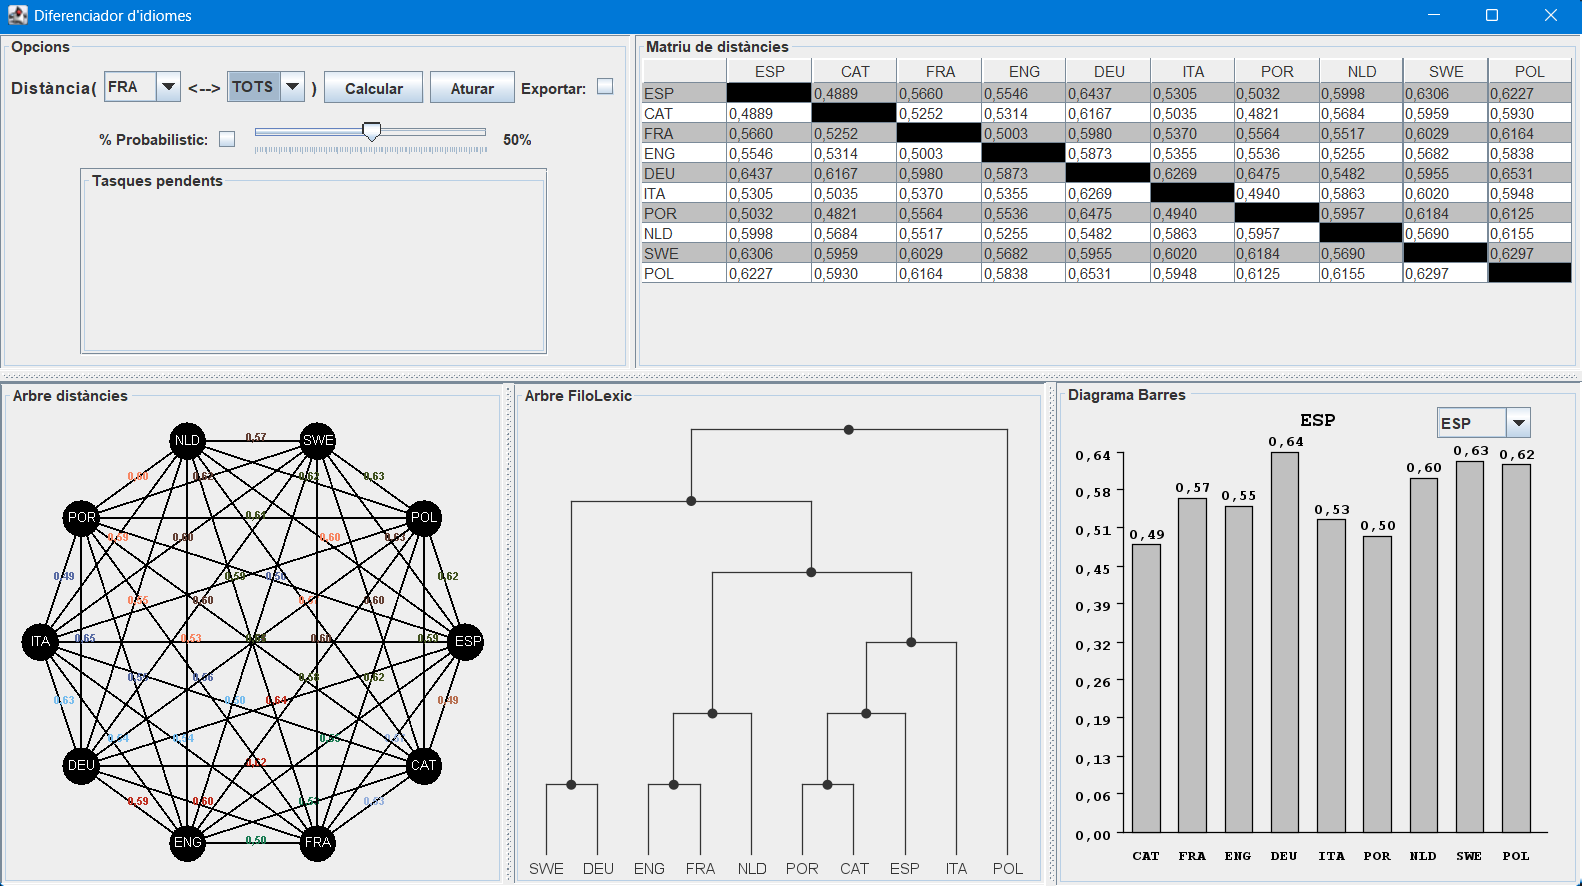
\includegraphics[width=0.8\linewidth, keepaspectratio]{png/finestraPrincipal.png}
        \caption{Finestra principal del programa}
        \label{fig:enter-label}
    \end{figure}
\end{itemize}


\subsection{Estructura de paquets i classes}
L'estructura del programa segueix les bones pràctiques d'encapsulament de Java. 
Els paquets principals es poden identificar d'acord amb el disseny de l'arquitectura Model-Vista-Controlador. 
La figura següent il·lustra l'estructura del nostre programa. \newline
Els quadres de colors representen diferents elements: \textcolor{blau}{els blaus}, les \textbf{classes}; \textcolor{gris}{els grisos}, les \textbf{interfícies};\textcolor{verd}{ i els altres}, els \textbf{paquets}.

\begin{figure}[H]
    \centering
    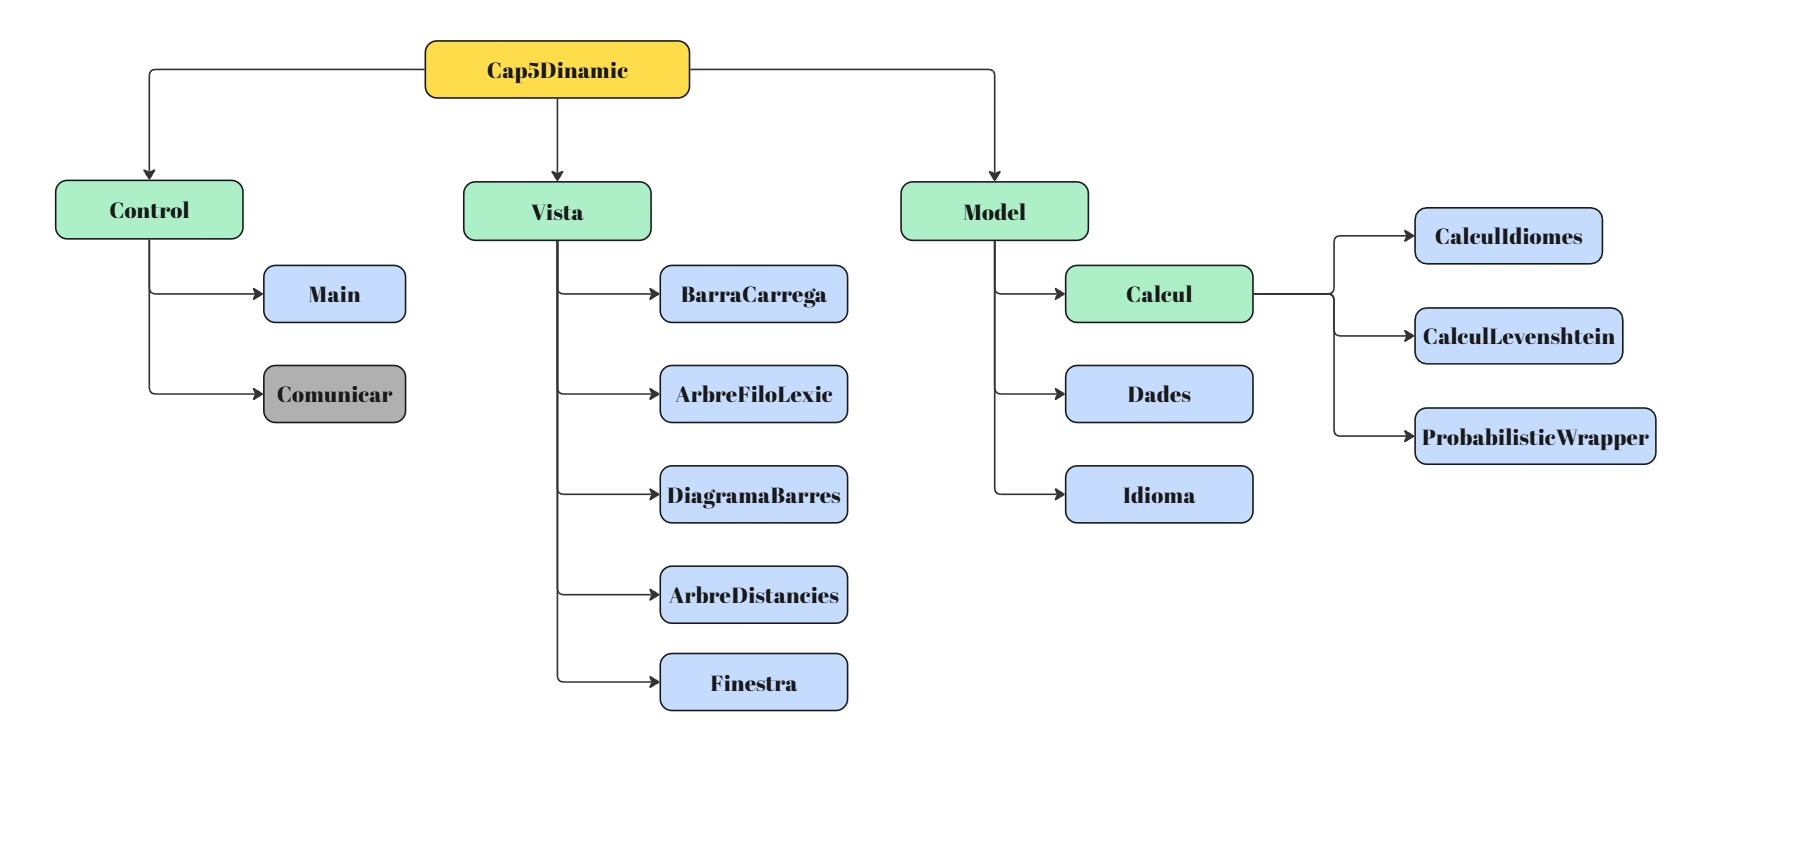
\includegraphics[width=\linewidth, keepaspectratio]{png/estructura.jpg}
    \caption{Estructura de paquets i classes }
    \label{fig:enter-label}
\end{figure}

\subsection{Algorisme de  Levenhstein} 

L’algorisme de Levenshtein s’implementa a la classe \texttt{CalculLevenshtein} (fitxer \texttt{CalculLevenshtein.java}) amb el mètode:
\begin{lstlisting}[language=Java]
// Classe: Model.CalculLevenshtein
public static int calcularDistanciaLevenshtein(String s1, String s2) {
    int n = s1.length(), m = s2.length();
    int[][] dp = new int[n+1][m+1];
    // Inicialització de casos base
    for (int i = 0; i <= n; i++) dp[i][0] = i;
    for (int j = 0; j <= m; j++) dp[0][j] = j;
    // Omplir matriu de costums
    for (int i = 1; i <= n; i++) {
        for (int j = 1; j <= m; j++) {
            int cost = (s1.charAt(i-1) == s2.charAt(j-1)) ? 0 : 1;
            dp[i][j] = Math.min(
                Math.min(dp[i-1][j] + 1, dp[i][j-1] + 1),
                dp[i-1][j-1] + cost
            );
        }
    }
    return dp[n][m];
}
\end{lstlisting}
Aquest codi segueix fidelment la formulació matemàtica:
\[
\begin{aligned}
dp[i][0] &= i,\quad dp[0][j] = j, \\
dp[i][j] &= \min\Bigl(
    dp[i-1][j] + 1,\;
    dp[i][j-1] + 1, \\
&\quad\quad\quad\;\;\;
    dp[i-1][j-1] + \delta(s_1[i], s_2[j])
\Bigr).
\end{aligned}
\]
on
\[
\delta(a,b)=
\begin{cases}
0,&a=b,\\
1,&a\neq b.
\end{cases}
\]
La distància final és $dp[n][m]$, que requereix temps $O(nm)$ i memòria $O(nm)$.

\subsection{Mètode de comparació d'Idiomes}
El càlcul global de la distància entre dos idiomes \(A\) i \(B\) es realitza a la classe \texttt{CalculIdiomes} (fitxer \texttt{CalculIdiomes.java}). Es defineix primer la distància dirigida:
\[
d(A\!\to\!B)
=
\frac{1}{|L_A|}
\sum_{w\in L_A}
\min_{x\in L_B}
\frac{\mathrm{Lev}(w,x)}{\max(|w|,|x|)},
\]
i després la distància simètrica:
\[
D(A,B)
=
\sqrt{\,d(A\!\to\!B)^2 + d(B\!\to\!A)^2\,}.
\]

\medskip
\noindent
\textbf{Concurrència:}  
S’empren dos \texttt{ExecutorService} per a calcular en paral·lel \(d(A\!\to\!B)\) i \(d(B\!\to\!A)\):
\begin{lstlisting}[language=Java]
// al constructor de CalculIdiomes
filsDistanci = Executors.newFixedThreadPool(2);
Future<Double> fAB = filsDistanci.submit(() -> calcularDistanciaOrdenat(A,B,true));
Future<Double> fBA = filsDistanci.submit(() -> calcularDistanciaOrdenat(B,A,false));
double dist = Math.hypot(fAB.get(), fBA.get());
\end{lstlisting}
Finalment s’afegeix la distància a l’objecte \texttt{Dades} per a posterior visualització.

\medskip
\noindent
\textbf{Pruning i partició de la llista:}  
El mètode \texttt{calcularDistanciaOrdenat} divideix el llistat de paraules en blocs segons el nombre de fils disponibles i, per a cada paraula, cerca la millor coincidència en el repertori de destí amb pruning basat en la diferència de longitud normalitzada:
\begin{lstlisting}[language=Java]
private double distanciaMin(String w, List<String> B) {
    // B està ordenat per longitud
    int pos = Collections.binarySearch(B, w, Comparator.comparingInt(String::length));
    // explorar creixent i decreixent fins a podar segons longitud
    ...
    int dist = calcularDistanciaLevenshtein(w, x);
    minim = Math.min(minim, dist/(double)Math.max(w.length(),x.length()));
    ...
}
\end{lstlisting}
Aquesta estratègia redueix el nombre de crides a l’algorisme de Levenshtein, mantenint l’exactitud de la distància.  

A més, si es trobés una distància igual a 0, al no existir una distància negativa, s'atura per la paraula en concret.

\subsection{Gestió de concurrència}
La gestió de la concurrència es realitza amb \texttt{ExecutorService}. Gràcies a l’ús d’aquest executor, es disposa d’un control dels fils simultanis mitjançant una cua d’espera.

Començant des de \texttt{Main}, s’utilitza \texttt{ExecutorService} per controlar el càlcul simultani de distàncies; per evitar sobrecàrregues, la mida del \emph{pool} és de 2 fils. A continuació, a \texttt{CalculIdiomes}, s’utilitzen tres \texttt{ExecutorService}: un per controlar les distàncies A-B i B-A, i dos més per a cada càlcul de distància respectivament.\newline

Amb l’executor assignat a cada càlcul de distàncies, les paraules es reparteixen equitativament entre els fils disponibles per, posteriorment, fer la composició dels resultats.


\subsection{Gestió probabilistic}
La gestió del mode probabilístic, mitjançant la tècnica de Monte Carlo~\cite{Montecarlo}, es duu a terme amb la classe \texttt{ProbabilisticWrapper}, que hereta de \texttt{CalculIdiomes} i modifica els mètodes d’obtenció de paraules per seleccionar-ne un percentatge del total. A més, repeteix el càlcul cinc vegades per reduir l’error.

Per exemple, el codi següent agafa un percentatge $X$ de paraules sense repetició.

\begin{lstlisting}[language=Java]
@Override
protected List<String> getParaules(Idioma x){
    List<String> orig = super.getParaules(x);
    List<String> paraulesRandom = new ArrayList<String>();
    Set<Integer> indexos = new TreeSet<>();
    Random r = new Random();
    while(indexos.size() < orig.size()*percent)
        indexos.add(r.nextInt(orig.size()));
    for(Integer i : indexos){
        paraulesRandom.add(orig.get(i));
    }
    return paraulesRandom;
}
\end{lstlisting}

\subsection{Visualització i interacció amb l'usuari}
La interfície gràfica d’usuari (GUI) s’ha desenvolupat amb la llibreria \texttt{Swing} i ha estat dissenyada per oferir una interacció senzilla, intuïtiva i funcional amb el model.
Els elements de visualització s'actualitzen automàticament al rebre noves dades

\paragraph{Estructura principal de la finestra}

La finestra principal (\texttt{Finestra}) està organitzada en cinc zones clarament diferenciades:
\begin{itemize}
   \item \textbf{Opcions}: conté botons i desplegables per a les accions bàsiques: \emph{Calcular}, \emph{Aturar} i \emph{Exportar}. Cada botó està associat a un \emph{listener} que desencadena una acció concreta mitjançant missatges enviats al controlador principal.\newline

Pel que fa als idiomes, hi ha dos desplegables, \emph{IdiomaA} i \emph{IdiomaB}, que permeten triar els idiomes per al càlcul de les distàncies. També inclouen l’opció \emph{TOTS}, que actua com a comodí per calcular diverses distàncies de manera eficient.

A més, hi ha un \emph{slider} acompanyat d’un \emph{checkbox} que permet configurar el mode probabilístic.\newline

Finalment, es disposa d’una secció amb barres de càrrega (\texttt{BarraCarrega}) que representen les tasques pendents. Aquestes permeten aturar tasques individuals i mostren el temps un cop finalitzades, oferint un retorn visual clar sobre l’activitat del programa en tot moment.\newline

    
    \item \textbf{Matriu de distàncies}: Mostra la matriu de distàncies dels diferents idiomes.
    \item \textbf{Gràfics i visualitzadors}: Visualitzen les dades amb tres diferents tipus de gràfics implementats.
    \begin{itemize}
       \item \textbf{Graf de distàncies}: Aquesta classe és responsable de la generació i l'actualització d'un arbre de distàncies entre els idiomes disponibles. Cada vegada que es guarda una nova distància a la matriu de distàncies, aquesta classe, gràcies al seu mètode \texttt{paintComponent}, actualitza automàticament la representació gràfica de l'arbre.\newline


A nivell d'implementació, el primer pas consisteix en calcular les posicions dels nodes, que es distribueixen de manera circular en funció de la mida actual del panell gràfic, garantint un representació visual equilibrada, independentment del nombre de nodes. 

Posteriorment, es dibuixen les connexions entre els idiomes seguint les distàncies calculades, aplicant diferents colors per millorar la llegibilitat del gràfic. Finalment, cada idioma es representa mitjançant un node identificable amb el seu nom i una etiqueta visual per facilitar-ne la interpretació.
\begin{lstlisting}
public void getPosicions() {

posicions = new Point[NODES];
for (int i = 0; i < NODES; i++) {
//per millor distribucio
double angle = 2 * Math.PI * i / NODES;
posicions[i] = new Point(CENTRE_X + (int) (RADI * Math.cos(angle)), CENTRE_Y + (int) (RADI * Math.sin(angle)));
        }
    }
\end{lstlisting}

A més, s’ha incorporat un mecanisme de verificació per assegurar que l’actualització del gràfic només es realitza quan la matriu conté distàncies vàlides i no nul·les, evitant redibuix innecessari i possibles inconsistències en la visualització.

        \begin{figure}[H]
            \centering
            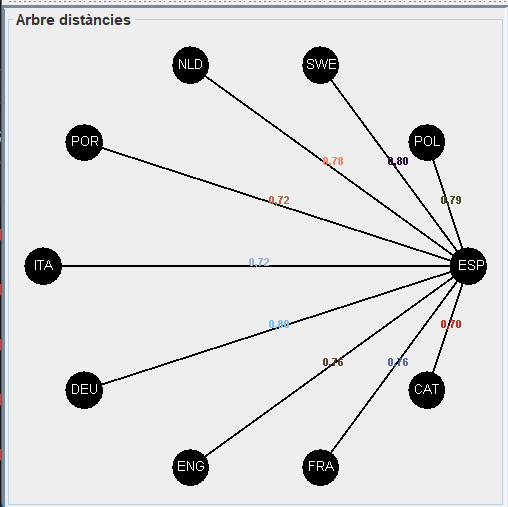
\includegraphics[width=0.5\linewidth]{png/image.png}
            \caption{Arbre de distàncies respecte al Espanyol (ESP)}
            \label{fig:enter-label}
        \end{figure}
        \item \textbf{Arbre filolèxic}: 
        s'encarrega de generar un arbre filo-lèxic basat en les distàncies entre idiomes i actualitzar-lo de manera dinàmica. En primer lloc, obté les distàncies entre idiomes de la classe \texttt{Dades} i construeix l'arbre jeràrquic utilitzant una agrupació progressiva de nodes, gestionada per la classe \texttt{Llista}. 
        
        \begin{lstlisting}[breaklines = true]
private static class Llista {
List<Node> llista;
double[][] distancies;
double[][] clusterDistances;

public Llista(double[][] distancies) {
    llista = new ArrayList<>();
    this.distancies = distancies;
}

//calcula la distancia entre dos nodes
public double getDistance(Node n1, Node n2) {
     List<Idioma> leaves1 = n1.getLeaves();
     List<Idioma> leaves2 = n2.getLeaves();
        double sum = 0.0;
      for (Idioma a : leaves1) {
        for (Idioma b : leaves2) {
            int idxA = a.ordinal();
            int idxB = b.ordinal();
            double d = (idxA > idxB) ? distancies[idxA][idxB] : distancies[idxB][idxA];
                sum += d;
                }
            }
    int count = leaves1.size() * leaves2.size();
return count > 0 ? sum / count : Double.MAX_VALUE;
    }
}
        \end{lstlisting}

       El mètode \texttt{getDistance(Node n1, Node n2)} calcula la distància mitjana entre dos nodes de l’arbre filo-lèxic basant-se en la matriu de distàncies \texttt{distancies[][]}. Primer, obté les fulles de cada node i recorre totes les combinacions possibles d’idiomes, acumulant les seves distàncies. La selecció del valor correcte es fa considerant la simetria de la matriu i, en cas de no tenir valors vàlids, retorna \texttt{Double.MAX\_VALUE}. \newline
       
       Aquest càlcul és essencial per fusionar nodes i establir la jerarquia de l’arbre, agrupant els idiomes en funció de la mínima distància fins a formar una estructura única. \newline
       
       Un cop acabat el càlcul, es distribueixen els nodes: les fulles es posicionen horitzontalment a la base del panell, mentre que els nodes interns es col·loquen en diferents nivells verticals en funció de la seva profunditat, assegurant una visualització clara i equilibrada. L’assignació de posicions es fa mitjançant una aproximació proporcional al nivell de profunditat dins l’arbre, calculant l’alçada de cada node respecte al màxim valor de distància trobat.\newline

        Quan el panell es redibuixa, \texttt{paintComponent(Graphics g)} comprova si la matriu de distàncies no estigui buida i, en aquest cas, executa \texttt{pintarArbreFiloLexic()}, garantint que només es pinta l’arbre quan les dades són definitives.
        \begin{figure}[H]
            \centering
            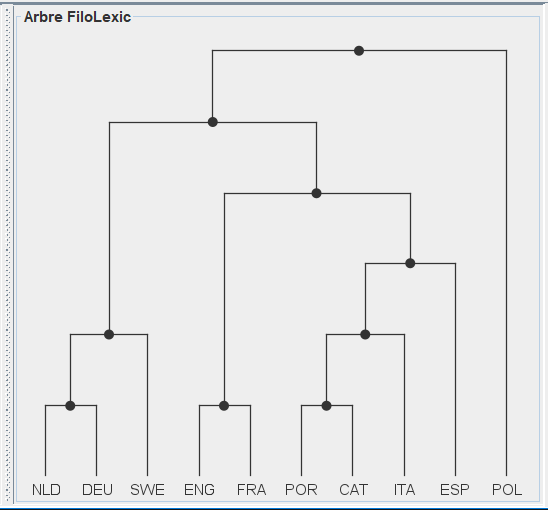
\includegraphics[width=0.5\linewidth]{png/arbreFilo.png}
            \caption{Exemple d'arbre filo-lèxic}
            \label{fig:enter-label}
        \end{figure}


     \item \textbf{Diagrama de barres}: Aquesta classe dibuixa un diagrama de barres per representar qualsevol distància calculada. 
        S'ha optat pel següent enfocament : primer es dibuixen els eixos amb els valors numèrics de la distància i, de manera automàtica, es posicionen els idiomes a l'eix horitzontal. Un cop s'afegeix una nova distància a la matriu de distàncies de la classe \textbf{Dades}, aquesta es reflecteix immediatament en el gràfic.
        Per facilitar l'ús, s'ha incorporat un botó que permet seleccionar l'idioma segons el qual es volen visualitzar les distàncies.
        \begin{figure}[H]
            \centering
            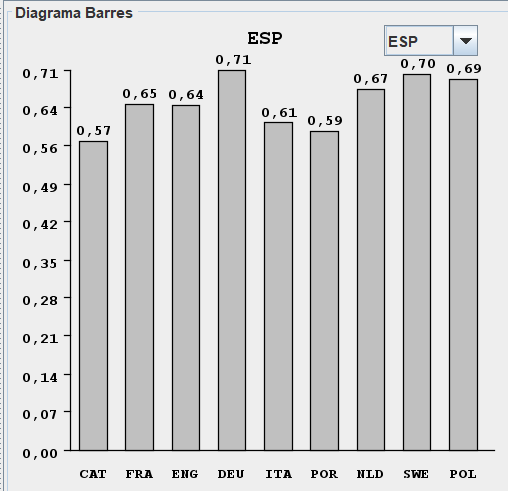
\includegraphics[width=0.5\linewidth]{png/diagramaB.png}
            \caption{Exemple de diagrama de barres respecte a l'espanyol}
            \label{fig:enter-label}
        \end{figure}
    \end{itemize}
\end{itemize}

Cal destacar que aquestes classes s'adapten dinàmicament a la mida real dels panells de la finestra principal, incloent-hi tots els seus elements gràfics.


\subsection{Decisions de disseny i extres implementats}
A nivell de disseny s'ha optat per modificar la interfície \texttt{Comunicar}, ara hi ha mètodes específics per a cada funció o missatge que es vol transmetre, a més, al utilitzar els \texttt{default} no totes les classes han d'implementar tots els mètodes.

De característiques extra implementades es pot destacar el següent:
\begin{itemize}
    \item \textbf{Gràfics de visualització} Permeten veure de forma gràfica els resultats.
     S'han implementat tres tipus diferents de gràfiques, com ja s'ha esmentat en seccions prèvies d'aquest document. Totes les gràfiques estenen \textbf{JPanel} i, gràcies al mètode \textit{paintComponent}, l'actualització dels resultats es fa de manera dinàmica. \newline

    Cap d'aquestes classes implementa la interfície \textbf{Comunicar}, ja que la informació necessària per a l'actualització del dibuix es pot obtenir directament a través de la matriu de distàncies. Cal remarcar \texttt{ArbreFilolexic} com a extra sol·licitat per a la pràctica.
    \item \textbf{Visualització dels processos} Quan s'efectua el càlcul d'una distància, s'afegeix a la finestra principal una barra de càrrega que simula l'execució del procés. Aquesta barra permet aturar el càlcul si és necessari i, un cop finalitzat, mostra el temps total que ha trigat a completar-se.\newline
    
    \item \textbf{Càlcul Probabilístic} Selecciona aleatòriament un percentatge de paraules del diccionari per reduir el càlcul final.
    L'usuari pot seleccionar, a través de la finestra principal del programa, si vol activar aquesta opció i amb quin percentatge, adaptant així el càlcul segons les seves necessitats.\newline
    
    \item \textbf{Càlcul Concurrent} Permet aprofitar els diferents fils del processador.\newline
    
  \item \textbf{Optimització del càlcul de distàncies}: preordena els diccionaris per longitud de paraula, mantenint l’ordre lèxic. La comparació comença amb paraules de la mateixa longitud i s’atura si la distància és zero o si s’assoleix un punt a partir del qual es pot garantir que no és possible obtenir un valor més petit.
    
    \item \textbf{Importar/Exportar}: L'usuari pot exportar els resultats dels càlculs de les distàncies en format \textbf{CSV} per reutilitzar-los en futures execucions o estudis. De la mateixa manera, és possible importar aquestes dades per analitzar-les i visualitzar-les dins de l'aplicació.
    
\end{itemize}



\section{Resultats i Comparació}
Abans de comentar els resultats, cal esmentar que tots els valors s’han obtingut amb el mode probabilístic activat, ja que el temps d’execució en mode determinista era inassumible, fins i tot amb les millores de tall implementades.

Aquesta és la matriu de distàncies amb un percentatge del 20\%:
\begin{figure}[H]
    \centering
    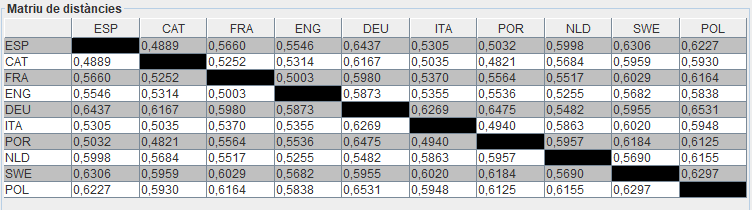
\includegraphics[width=\linewidth]{png/20p.png}
    \caption{Matriu de dades}
    \label{fig:enter-label}
\end{figure}
A continuació es mostren les diferents gràfiques generades amb aquestes dades.

\begin{figure}[H]
    \centering
    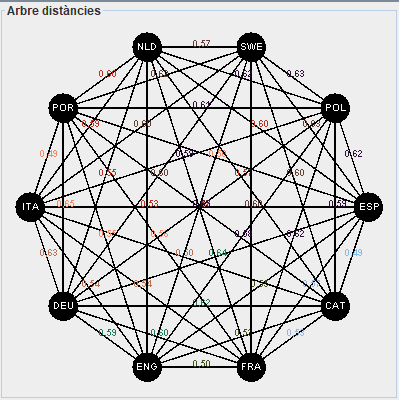
\includegraphics[width=\linewidth]{png/graf.png}
    \caption{Graf de distàncies}
    \label{fig:enter-label}
\end{figure}

Amb l’arbre filolèxic es poden visualitzar ràpidament les similituds relatives entre els idiomes. Com és d’esperar, les llengües que pertanyen a famílies properes apareixen més properes dins l’arbre que aquelles que no tenen una relació lingüística directa.

\begin{figure}[H]
    \centering
    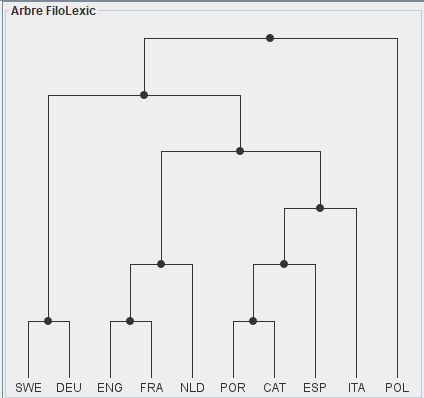
\includegraphics[width=\linewidth]{png/imagen.png}
    \caption{Arbre filolexic}
    \label{fig:enter-label}
\end{figure}

Com es pot observar al diagrama de barres, les llengües romàniques presenten una distància més propera al català en comparació amb les que no ho són. Destaquen el castellà i el portuguès com les més properes, mentre que l’alemany es troba entre les més llunyanes.

\begin{figure}[H]
    \centering
    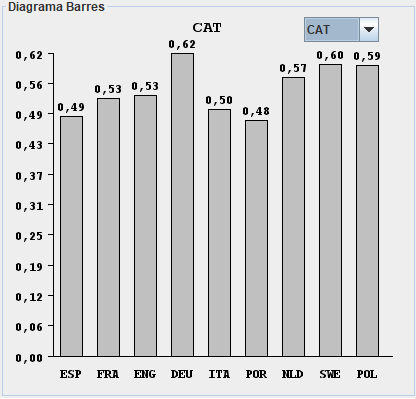
\includegraphics[width=\linewidth]{png/barres.png}
    \caption{Diagrama de barres per al català}
    \label{fig:enter-label}
\end{figure}

Per acabar, es mostra una comparativa de certes distàncies obtingudes amb el càlcul determinista, amb el mode probabilístic al 20\% i al 5\%.
\begin{table}[H]
    \centering
    \begin{tabular}{|l|l|l|l|}
        \hline
        \textbf {Idioma} & \textbf{Determinista} & \textbf{20\% } & \textbf{5\%} \\
        \hline
         ESP-ENG	 &0.4298 &0.5546	&0.6558 \\
         ITA-ESP	 &0.4195	 &0.6020	&0.6210 \\
         POR-FRA	 &0.4481 &0.5564	&0.6460 \\
        \hline
    \end{tabular}
    \vspace{3mm}
    \caption{Taula de la diferència dels valors segons el percentatge}
\end{table}

I els temps d'execució per a cada mètode, en segons:
\begin{table}[H]
    \centering
    \begin{tabular}{|l|l|l|l|}
        \hline
        \textbf {Idioma} & \textbf{Determinista} & \textbf{20\% } & \textbf{5\%} \\
        \hline
         ESP-ENG	 &299.54	&53.51	&3.47 \\
         ITA-ESP	 &241.27	&162.67	&7.71 \\
         POR-FRA	 &1319.41	&217.03	&12.26 \\
        \hline
    \end{tabular}
    \vspace{3mm}
    \caption{Taula de la diferència dels temps segons el percentatge}
\end{table}

Com es pot observar, a mesura que augmenta el percentatge del mode probabilístic, el valor obtingut s'aproxima més al càlcul determinista. Tanmateix, l'ús del mode probabilístic permet un estalvi significatiu en el temps d'execució.

Tot i així, mentre que la comparació de valors concrets pot oferir una idea general, si analitzam les gràfiques que representen tots els idiomes amb percentatges del 20\% i del 5\%, respectivament, podem observar que, encara que els valors absoluts variïn, es manté la relació entre les distàncies.

Per tant, com a conclusió, podem afirmar que, per aquest problema, l'ús de mètodes probabilístics permet obtenir resultats coherents, tot i que no siguin del tot precisos.


Hi ha una tendència a distancies més grans, això pot explicar-se que amb un menor percentatge, és més probable no triar un parell de paraules amb distància mínima, quedant només amb qui te més distància. 
\begin{figure}[H]
    \centering
    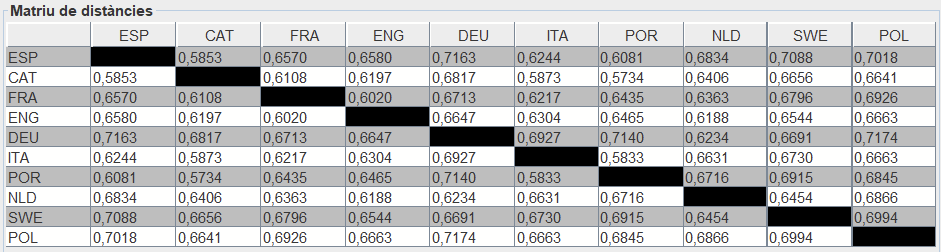
\includegraphics[width=\linewidth]{png/taula5.png}
    \caption{Matriu de dades amb 5\%}
    \label{fig:enter-label}
\end{figure}

Es cert que hi ha diferències, però els diferents grups d'idiomes es mantenen junts o molt prop que al de 20\% 
\begin{figure}[H]
    \centering
    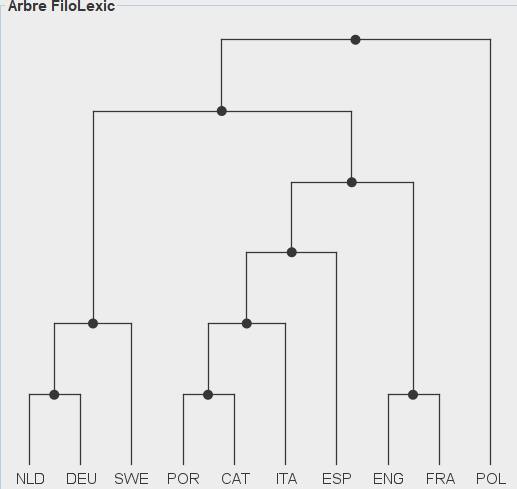
\includegraphics[width=\linewidth]{png/filolexic5.png}
    \caption{Arbre filo-lèxic amb 5\%}
    \label{fig:enter-label}
\end{figure}

Sense la presència de valors numèrics, seria difícil distingir quina figura correspon al 5\% i quina al 20\%.

\begin{figure}[H]
    \centering
    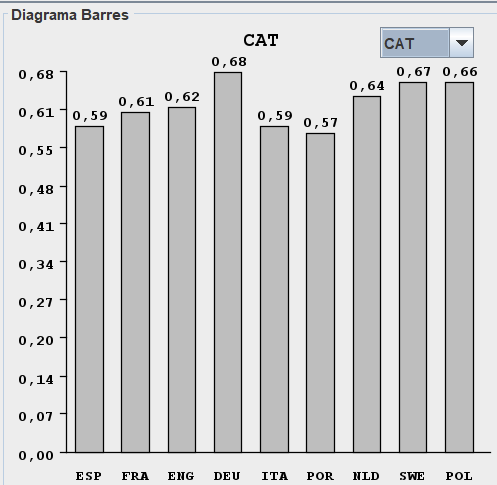
\includegraphics[width=\linewidth]{png/barres5p.png}
    \caption{Diagrama de barres}
    \label{fig:enter-label}
\end{figure}
\section{Conclusions}

En conclusió, tenim una bona visió d'aquesta pràctica, s’ha pogut implementar la funcionalitat inicialment plantejada. A més, ha estat molt enriquidor comprovar com diverses optimitzacions —com l’ús de concurrència, tècniques de poda, entre d’altres— han reduït considerablement el temps d’execució. Tot i això, per a diccionaris de gran mida, el temps de càlcul continua sent inviable amb els ordinadors disponibles.

Des d’un punt de vista personal, ha estat especialment interessant constatar, un cop més, la utilitat de la informàtica en tasques que inicialment podrien semblar fora de l’abast dels programes.

Pel que fa al treball en equip, consideram que aquesta pràctica ha funcionat millor per diversos motius. En primer lloc, la incorporació d’una nova interfície, \texttt{Comunicar}, ha facilitat una integració més robusta entre les diferents parts del projecte. A més, la nova organització temporal de les tasques ha permès un desenvolupament més sincronitzat, evitant problemes importants de coordinació.

Finalment, a continuació es presenta una figura que il·lustra el repartiment de tasques durant aquesta pràctica.


\begin{figure}[H]
    \centering
    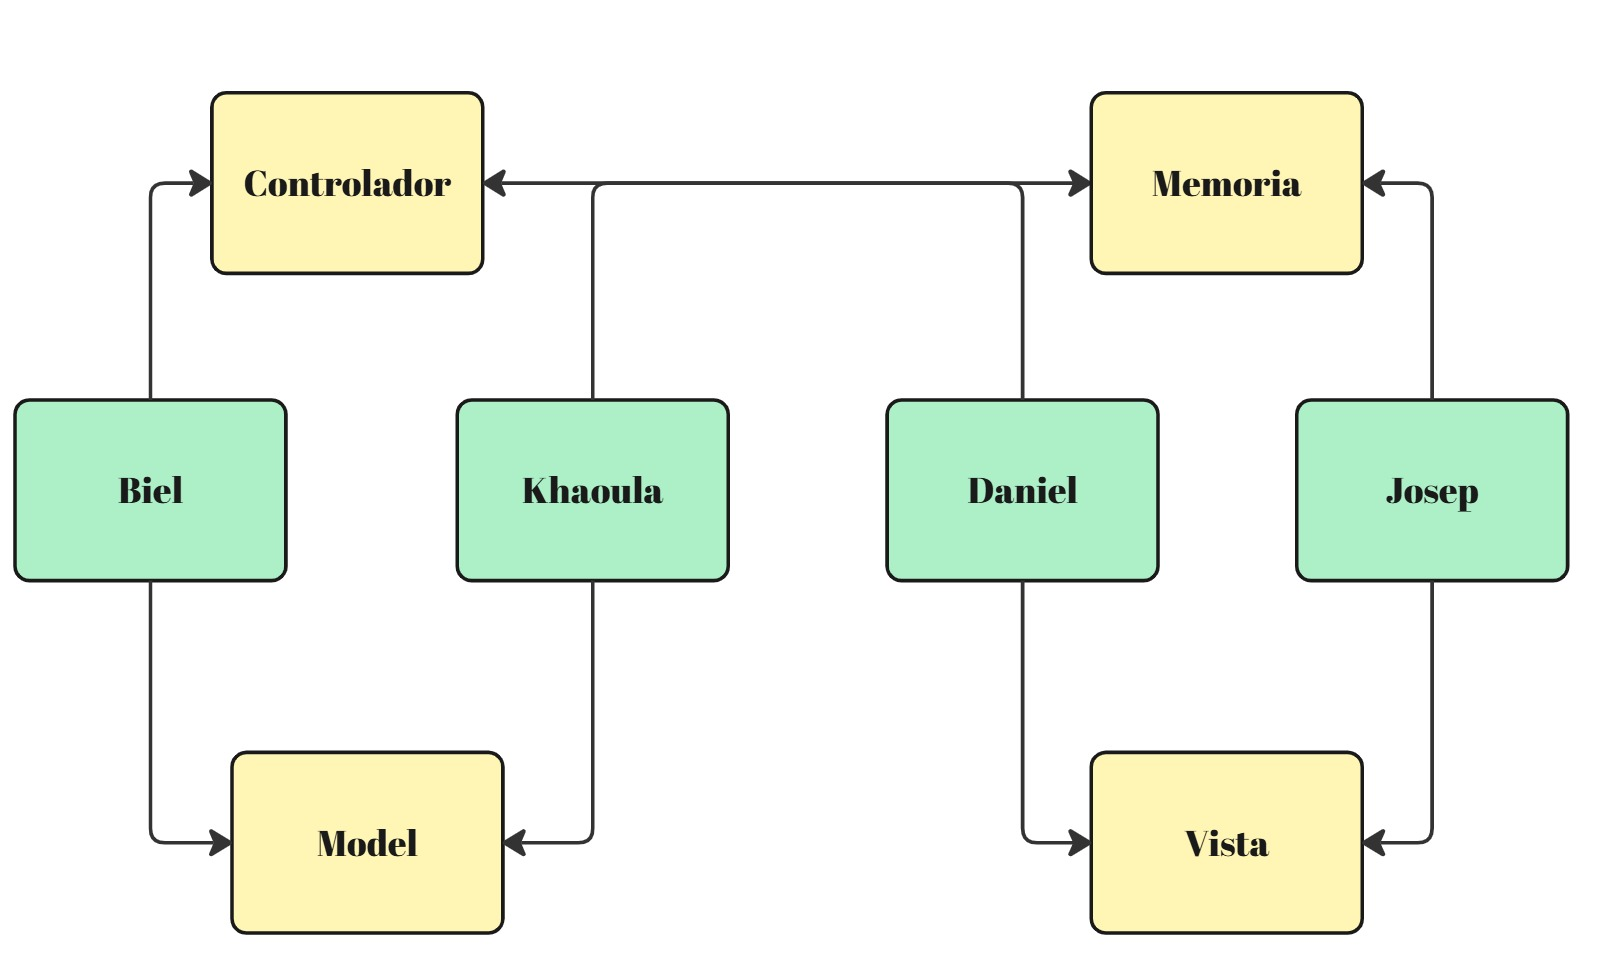
\includegraphics[width=0.5\linewidth]{png/Repartiment.jpg}
    \caption{Repartiment de tasques}
    \label{fig:enter-label}
\end{figure}

\bibliographystyle{plain}
\begin{thebibliography}{9}

\bibitem{IndoEuropeanLanguages}
Wikipedia contributors, \textit{Lenguas indoeuropeas}, Wikipedia, La enciclopedia libre. Disponible en: \url{https://es.wikipedia.org/wiki/Lenguas_indoeuropeas} [Último acceso: mayo 2025].

\bibitem{LevenshteinDistance}
Wikipedia contributors, \textit{Distancia de Levenshtein}, Wikipedia, La enciclopedia libre. Disponible en: \url{https://es.wikipedia.org/wiki/Distancia_de_Levenshtein} [Último acceso: mayo 2025].

\bibitem{MVC_Theory}
T. Reenskaug, \textit{The Model-View-Controller (MVC) Pattern}, Software Engineering Notes, vol. 10, no. 6, pp. 1–3, Dec. 1985.

\bibitem{mvcPattern}
GeeksforGeeks. (2021). \textit{MVC Design Pattern}. \\ \url{https://www.geeksforgeeks.org/mvc-design-pattern/}.

\bibitem{SwingLibrary}
Oracle, \textit{Swing: A GUI Widget Toolkit}, Oracle Corporation, 2009. \\ \url{https://docs.oracle.com/javase/8/docs/api/javax/swing/package-summary.html}.

\bibitem{oracleExecutorService}
Oracle. (2014). \textit{ExecutorService Interface (Java Platform SE 8)}. \\ \url{https://docs.oracle.com/javase/8/docs/api/java/util/concurrent/ExecutorService.html}.

\bibitem{DPConcept}
T. H. Cormen et al., \textit{Introduction to Algorithms}, 3rd ed. MIT Press, 2009.

\bibitem{levDistanceWiki}
Wikipedia. \textit{Levenshtein distance}. \\ \url{https://en.wikipedia.org/wiki/Levenshtein_distance}.

\bibitem{Navarro}
G. Navarro, “A guided tour to approximate string matching,” ACM Computing Surveys, vol. 33, no. 1, pp. 31–88, 2001.

\bibitem{phyloClustering}
J. Felsenstein, \textit{Inferring Phylogenies}. Sinauer Associates, 2004.

\bibitem{Montecarlo}
Wikipedia. \textit{Metode de montecarlo} \url{https://es.wikipedia.org/wiki/M%C3%A9todo_de_Montecarlo}, 2025.

\end{thebibliography}

\end{document}


